\documentclass{article}
\usepackage{main} % 加载自定义的 sty 文件
\usepackage[utf8]{inputenc}
\usepackage{xcolor}
\usepackage{ctex}
\usepackage{amsmath}
\usepackage{amsfonts}
\usepackage{amssymb}
\usepackage{geometry}
\geometry{a4paper, margin=1in}
\usepackage{enumitem}
\usepackage{pifont} 
\renewcommand{\arraystretch}{1.5}
\usepackage{longtable} 
\usepackage{mdframed}
\usepackage{tabularx}
\usepackage{graphicx}
\usepackage[backend=biber,style=ieee,dashed=false,url=false,isbn=false,defernumbers=false]{biblatex}
\definecolor{chapterbg}{RGB}{0,153,102} 
\definecolor{guidelightbg}{RGB}{230,245,235}
\definecolor{exercisemark}{RGB}{255,153,0}  
\usepackage{tikz}
\usetikzlibrary{decorations.pathmorphing}
\usetikzlibrary{decorations.pathmorphing, decorations.pathreplacing}
\addbibresource{literature.bib}


\begin{document}

% Response to the reviewers
\noindent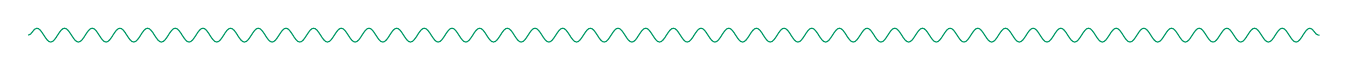
\begin{tikzpicture}
  \draw[decoration=snake, chapterbg, decorate] (0,0) -- (16.4,0);
\end{tikzpicture}
\begin{center}
\colorbox{chapterbg}{\textcolor{white}{\Large\textbf{Responses to Reviewers' Comments}}}
\end{center}
\noindent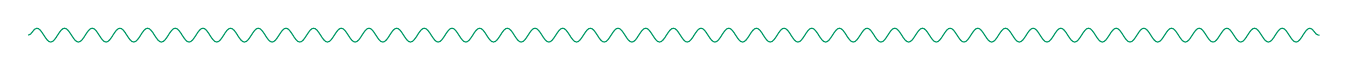
\begin{tikzpicture}
  \draw[decoration=snake, chapterbg, decorate] (0,0) -- (16.4,0);
\end{tikzpicture}
\vspace{1em}

\noindent\colorbox{guidelightbg}{%
\noindent\begin{minipage}{\linewidth}
\begin{itemize}[leftmargin=*, label=$\Box$] 
\item {\color{blue}\textbf{Manuscript ID:}}~ <Manuscript ID>
\item {\color{blue}\textbf{Title:}}~ <Manuscript Title>
\item {\color{blue}\textbf{Author:}}~ <Author Names>
\end{itemize}
\end{minipage}
}\\[1em]

\noindent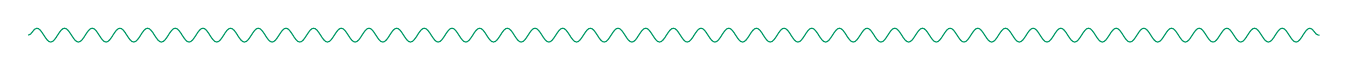
\begin{tikzpicture}
  \draw[decoration=snake, chapterbg, decorate] (0,0) -- (16.4,0);
\end{tikzpicture}
To Editor and Reviewers:

<Your response to the editor and reviewers, including a brief summary of the major revisions made to the manuscript.>


\noindent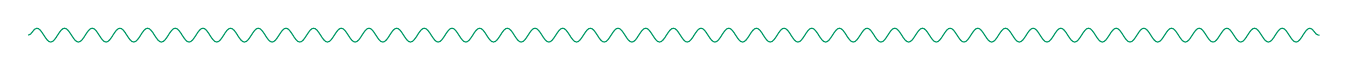
\begin{tikzpicture}
  \draw[decoration=snake, chapterbg, decorate] (0,0) -- (16.4,0);
\end{tikzpicture}
\clearpage



%%%%%%%%%%%%%%%%%%%%有几个审稿人在《结束》前复制几个以下组件%%%%%%%%%%%%%%%%%%%%%%%%%%%%%%
\noindent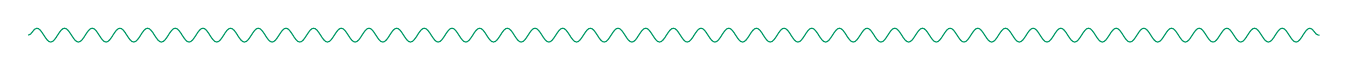
\begin{tikzpicture}
  \draw[decoration=snake, chapterbg, decorate] (0,0) -- (16.4,0);
\end{tikzpicture}
\begin{center}
\Large\textbf{\textcolor{chapterbg}{Reviewer 1}} %注意修改为实际的审稿人编号
\end{center}
\noindent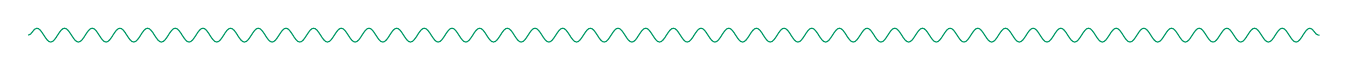
\begin{tikzpicture}
  \draw[decoration=snake, chapterbg, decorate] (0,0) -- (16.4,0);
\end{tikzpicture}
\vspace{1em}
\input{reviews/R1.tex} %注意修改为实际的审稿人意见文件路径
%%%%%%%%%%%%%%%%%%%%%%%%%%%%%%%%%%%%%%%%%%%%%%%%%%%%%%%%%%%%%%%%%%%%%%%%%%%%%%%%%%%%%%%

% 审稿人2


% 审稿人3


%%%%%%%%%%%%%%%%%%%%%结束%%%%%%%%%%%%%%%%%%%%%%%%%%%%%%%

\noindent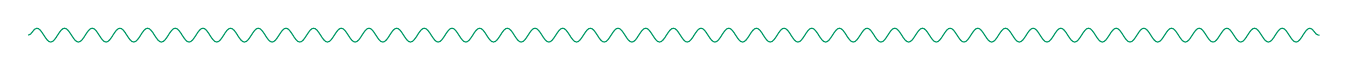
\begin{tikzpicture}
  \draw[decoration=snake, chapterbg, decorate] (0,0) -- (16.4,0);
\end{tikzpicture}

<总结，感谢编辑和评审的意见，并强调你对这些意见的重视，以及你对改进论文的承诺。若无必要，则删除此段。>

\noindent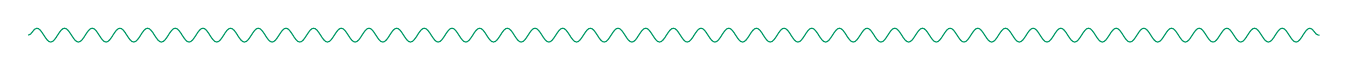
\begin{tikzpicture}
  \draw[decoration=snake, chapterbg, decorate] (0,0) -- (16.4,0);
\end{tikzpicture}
\clearpage
\printbibliography[heading=bibintoc, heading=bibliography, title={References}, section=\therefsection]
%%%%%%%%%%%%%%%%%%%%%%%%%%%%%%%%%%%%%%%%%%%%%%%%%%%%%%%%%%%
\end{document} 
%%%%%%%%%%%%%%%%%%%%%%%%%%%%%%%%%%%%%%%%%%%%%%%%%%%%%%%%%%%